\documentclass[10pt,letterpaper, cm]{hmcpset}
\usepackage[top=0.5in,bottom=1in,right=1in,left=0.75in]{geometry}
\usepackage{multicol,graphicx, enumerate, cancel, amsmath, amsthm}
\usepackage{tikz}
\usepackage{tikz,fullpage}

\usetikzlibrary{arrows,petri,topaths}
				
\usepackage{tkz-berge}
\usepackage{tkz-graph}

\name{Jonathon Sonesen}
\class{CS 251}
\duedate{\today}
\assignment{Graph Theory Knowledge}
\extraline{Collaborators:Jeff Patterson, Steven Wetherebee, Kyle Kneitenger}

%% column seperation options for multicol
\setlength{\columnsep}{0.5cm}
\setlength{\columnseprule}{00pt}

%%% Macros:

\newcommand{\nn}{\sim\!\!} % logical not operator that sits close to its operand

\newcommand{\lp}{\left(}
\newcommand{\rp}{\right)}
\newcommand{\lbk}{\left[}
\newcommand{\rbk}{\right]}
\newcommand{\lbr}{\left\lbrace}
\newcommand{\rbr}{\right\rbrace}
\newcommand{\defn}{\text{by def. of }}
\newcommand{\alg}{\text{algebra}}
\newcommand{\stdsum}{\sum_{i=1}^{n}}
\newcommand{\RA}{\Rightarrow}
\renewcommand{\qed}{\quad\ensuremath{\scriptscriptstyle\blacksquare}}
\newcommand{\inprime}{\in \mathbb{Z}^{\mathbb{P}}}
\newcommand{\ninprime}{\notin \mathbb{Z}^{\mathbb{P}}}
\newcommand{\inints}{\in \mathbb{Z}}
\newcommand{\inreals}{\in \mathbb{R}}
\newcommand{\st}{\;\;\Big|\;\;}
%%%%


\begin{document}


\section*{Graph Theory Knowledge Assignment}

\begin{problem}[1]

  Let $G$ be a simple graph with $n$ nodes. 
  Let $k$ be the number of edges of $G$. Prove (or disprove)
  \[k \leq \frac{n(n-1)}{2}\]
\end{problem}

\begin{problem}[2]

  Let $G$ be the graph:

  \begin{center}
      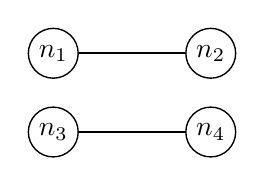
\begin{tikzpicture}[scale=1,transform shape]
        \GraphInit[vstyle=Dijkstra]
        \SetVertexMath

        \Vertex[x=0,y=0]{n_1}
        \Vertex[x=2,y=0]{n_2}
        \Vertex[x=0,y=-1]{n_3}
        \Vertex[x=2,y=-1]{n_4}
        \Edge[](n_1)(n_2)
        \Edge[](n_3)(n_4)
    \end{tikzpicture}
  \end{center}
What is the complement of $G$?
\end{problem}

\begin{problem}[3]
List a simple graph that has 4 nodes of different degrees, or prove that no such graph exists.
\end{problem}

\begin{problem}[4]
What is the maximum number of edges possible in a disconnected graph with $n$ nodes and no loops or parallel edges?  Explain your answer. (No proof needed)
\end{problem}

\begin{problem}[5]
Let $G$ be the graph:


\begin{center}

    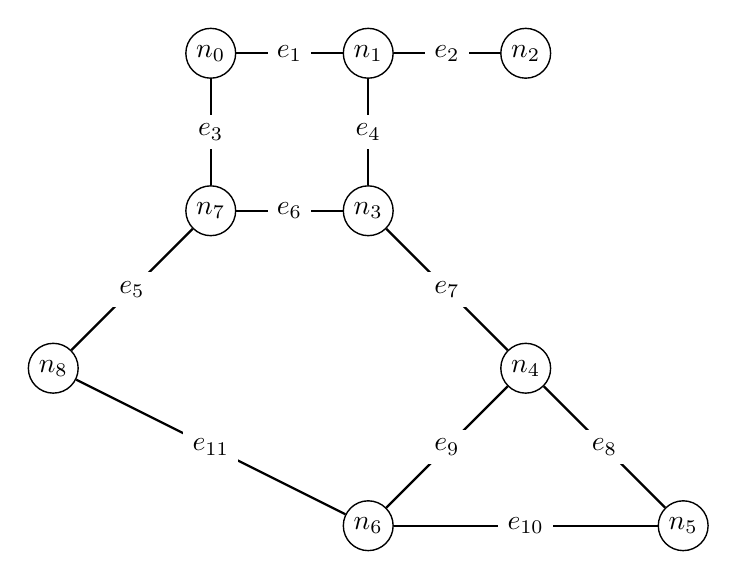
\begin{tikzpicture}[scale=1,transform shape]

        \GraphInit[vstyle=Dijkstra]

        \SetVertexMath
        \Vertex[x=0, y=0]{n_0}
        \Vertex[x=2, y=0]{n_1}
        \Vertex[x=4, y=0]{n_2}
        \Vertex[x=2, y=-2]{n_3}
        \Vertex[x=4, y=-4]{n_4}
        \Vertex[x=6, y=-6]{n_5}
        \Vertex[x=2, y=-6]{n_6}
        \Vertex[x=0, y=-2]{n_7}
        \Vertex[x=-2, y=-4]{n_8}
        \Edge[label=$e_1$](n_0)(n_1)
        \Edge[label=$e_2$](n_1)(n_2)
        \Edge[label=$e_3$](n_0)(n_7)
        \Edge[label=$e_4$](n_1)(n_3)
        \Edge[label=$e_5$](n_7)(n_8)
        \Edge[label=$e_6$](n_7)(n_3)
        \Edge[label=$e_7$](n_3)(n_4)
        \Edge[label=$e_8$](n_4)(n_5)
        \Edge[label=$e_9$](n_4)(n_6)
        \Edge[label=$e_{10}$](n_6)(n_5)
        \Edge[label=$e_{11}$](n_6)(n_8)

    \end{tikzpicture}
\end{center}

\begin{enumerate}[(a)]
    \item List the Adjacency matrix for this graph
    \item List the Incidence matrix for this graph
\end{enumerate}
\end{problem}

\begin{problem}[6]
    Let $G$ be the graph:

    \begin{center}
    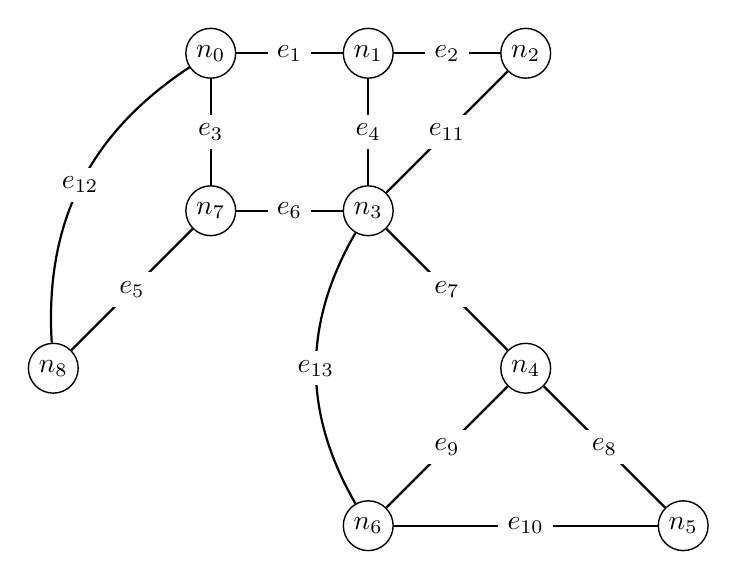
\begin{tikzpicture}[scale=1,transform shape]
        \GraphInit[vstyle=Dijkstra]
        \SetVertexMath

        \Vertex[x=0, y=0]{n_0}
        \Vertex[x=2, y=0]{n_1}
        \Vertex[x=4, y=0]{n_2}
        \Vertex[x=2, y=-2]{n_3}
        \Vertex[x=4, y=-4]{n_4}
        \Vertex[x=6, y=-6]{n_5}
        \Vertex[x=2, y=-6]{n_6}
        \Vertex[x=0, y=-2]{n_7}
        \Vertex[x=-2, y=-4]{n_8}
        \Edge[label=$e_1$](n_0)(n_1)
        \Edge[label=$e_2$](n_1)(n_2)
        \Edge[label=$e_3$](n_0)(n_7)
        \Edge[label=$e_4$](n_1)(n_3)
        \Edge[label=$e_5$](n_7)(n_8)
        \Edge[label=$e_6$](n_7)(n_3)
        \Edge[label=$e_7$](n_3)(n_4)
        \Edge[label=$e_8$](n_4)(n_5)
        \Edge[label=$e_9$](n_4)(n_6)
        \Edge[label=$e_{10}$](n_6)(n_5)
        \Edge[label=$e_{11}$](n_3)(n_2)
        \Edge[style={bend right}, label= $e_{12}$](n_0)(n_8)
        \Edge[style={bend right}, label= $e_{13}$](n_3)(n_6)

    \end{tikzpicture}
    \end{center}

    \begin{enumerate}[(a)]
        \item List the Laplacian matrix for this graph
        \item List the eigenvalues for the Laplacian matrix for this graph
    \end{enumerate}
\end{problem}

\begin{problem}[7]
    Let $G$ be the graph:

    \begin{center}
    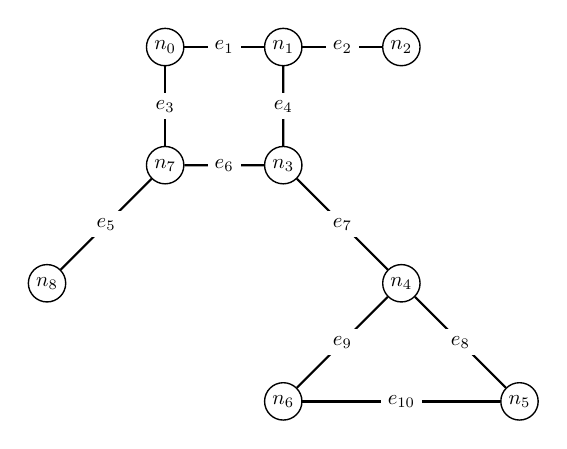
\begin{tikzpicture}[scale=.75, transform shape]
        \GraphInit[vstyle=Dijkstra]
        \SetVertexMath

        \Vertex[x=0, y=0]{n_0}
        \Vertex[x=2, y=0]{n_1}
        \Vertex[x=4, y=0]{n_2}
        \Vertex[x=2, y=-2]{n_3}
        \Vertex[x=4, y=-4]{n_4}
        \Vertex[x=6, y=-6]{n_5}
        \Vertex[x=2, y=-6]{n_6}
        \Vertex[x=0, y=-2]{n_7}
        \Vertex[x=-2, y=-4]{n_8}
        \Edge[label=$e_1$](n_0)(n_1)
        \Edge[label=$e_2$](n_1)(n_2)
        \Edge[label=$e_3$](n_0)(n_7)
        \Edge[label=$e_4$](n_1)(n_3)
        \Edge[label=$e_5$](n_7)(n_8)
        \Edge[label=$e_6$](n_7)(n_3)
        \Edge[label=$e_7$](n_3)(n_4)
        \Edge[label=$e_8$](n_4)(n_5)
        \Edge[label=$e_9$](n_4)(n_6)
        \Edge[label=$e_{10}$](n_6)(n_5)

    \end{tikzpicture}
    \end{center}

    \begin{enumerate}[(a)]
        \item List the Degree matrix for this graph
        \item List the Adjacency matrix for this graph
        \item Identify the bridges (if any) of this graph. If ther are no bridges, write ``none''.
    \end{enumerate}
\end{problem}

\begin{problem}[8]
    Let $G$ be the graph:
    
    \begin{center}
    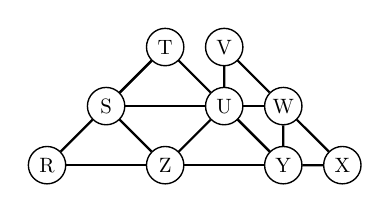
\begin{tikzpicture}[scale=.75, transform shape]
        \GraphInit[vstyle=Dijkstra]
        \SetGraphUnit{1}

        \Vertex{T} \EA(T){V}
        \SOWE(T){S} \SOEA(T){U} \SOEA(V){W}
        \SOWE(S){R} \SOWE(U){Z} \SOEA(U){Y} \SOEA(W){X}
        \Edges(T,S,R,Z,S,U,Z,Y,U,S,T,U,Y,X,W,Y,U,W,V,U)

    \end{tikzpicture}
    \end{center}

    \begin{enumerate}[(a)]
        \item List the Laplacian matrix for this graph
        \item List the Incidence matrix for this graph
        \item Identify an Euler circuit for this graph, or prove no such circuit exists
    \end{enumerate}
\end{problem}

\begin{problem}[9]
    Let $G$ be the graph:
    \begin{center}
    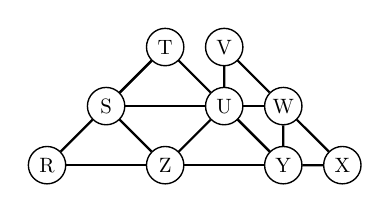
\begin{tikzpicture}[scale=.75, transform shape]
        \GraphInit[vstyle=Dijkstra]
        \SetGraphUnit{1}

        \Vertex{T} \EA(T){V}
        \SOWE(T){S} \SOEA(T){U} \SOEA(V){W}
        \SOWE(S){R} \SOWE(U){Z} \SOEA(U){Y} \SOEA(W){X}
        \Edges(T,S,R,Z,S,U,Z,Y,U,S,T,U,Y,X,W,Y,U,W,V,U)

    \end{tikzpicture}
    \end{center}

    \begin{enumerate}[(a)]
        \item List the Adjacency matrix for this graph
        \item List the Degree matrix for this graph
        \item Identify a Hamiltonian circuit for this graph, or prove no such circuit exists
    \end{enumerate}
\end{problem}

\begin{problem}[10]
    Let $G$ be the graph:
    \begin{center}
    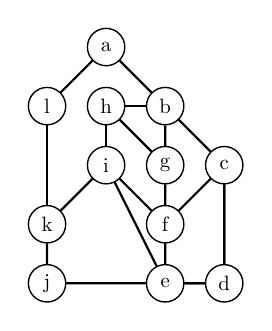
\begin{tikzpicture}[scale=.75, transform shape]
        \GraphInit[vstyle=Dijkstra]
        \SetGraphUnit{1}

        \Vertex{a} \SOWE(a){l} \SO(a){h} \SOEA(a){b}
	\SO(h){i} \SO(b){g} \SOEA(b){c}
	\SOWE(i){k} \SOEA(i){f}
	\SO(k){j} \SO(f){e} \SOEA(f){d}
        \Edges(a,l,k,j,e,d,c,b,a)
        \Edges(k,i,h,b,g,h,i,f,c,d,e,i)
        \Edges(e,f,g)
    \end{tikzpicture}
    \end{center}

    \begin{enumerate}[(a)]
        \item List the Adjacency matrix for this graph
        \item List the Degree matrix for this graph
        \item Identify an Euler circuit for this graph, or prove no such circuit exists
    \end{enumerate}
\end{problem}

\begin{problem}[11]
    Let $G$ be the graph:
    \begin{center}
    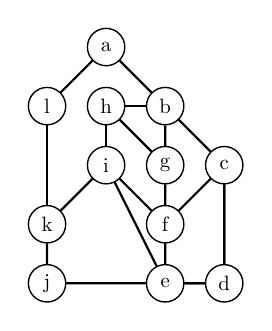
\begin{tikzpicture}[scale=.75, transform shape]
        \GraphInit[vstyle=Dijkstra]
        \SetGraphUnit{1}

        \Vertex{a} \SOWE(a){l} \SO(a){h} \SOEA(a){b}
	\SO(h){i} \SO(b){g} \SOEA(b){c}
	\SOWE(i){k} \SOEA(i){f}
        \SO(k){j} \SO(f){e} \SOEA(f){d}
        \Edges(a,l,k,j,e,d,c,b,a)
        \Edges(k,i,h,b,g,h,i,f,c,d,e,i)
        \Edges(e,f,g)

    \end{tikzpicture}
    \end{center}

    \begin{enumerate}[(a)]
        \item List the Laplacian matrix for this graph
        \item List the Incidence matrix for this graph
        \item Identify a Hamiltonian circuit for this graph, or prove no such circuit exists
        \end{enumerate}
\end{problem}

\newpage


    \begin{center}
    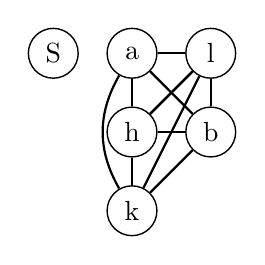
\begin{tikzpicture}[scale=1, transform shape]
        \GraphInit[vstyle=Dijkstra]
        \SetGraphUnit{1}

        \Vertex{a} \EA(a){l} \SO(a){h} \SOEA(a){b}
	\SO(h){k} \WE(a){S}
        \Edges(a,l,h,a,b)
        \Edge[style={bend right}](a)(k)
        \Edges(l,h,b,l)
        \Edges(h,k,b)
        \Edges(k,l)
    \end{tikzpicture}

    \begin{align*}
        k &\leq \frac{(n-1)((n-1)-1)}{2}
    \end{align*}
    \end{center}

\end{document}
